When opening \emph{Flat Hunt} in EiffelStudio, the cluster view in the bottom left corner of EiffelStudio shows many clusters. For you only the top-level clusters \emph{Traffic} and \emph{Flat\_hunt} are important.\\

To remove complexity, \emph{Flat Hunt} is structured in four top-level (see \autoref{flat_hunt_clusters}): \emph{Model}, \emph{View}, \emph{Controller} and \emph{Util}. Some clusters contain sub-clusters and in each cluster there are several classes.

\begin{figure}[h]
\centerline{\hbox{  
  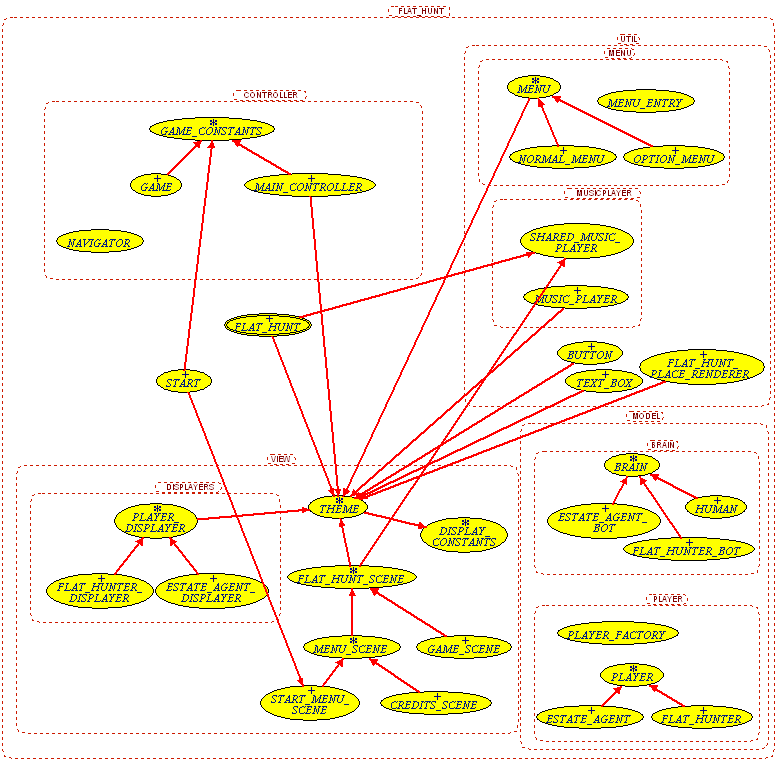
\includegraphics[width=135mm]{flat_hunt_clusters}
  }}
\caption{Flat Hunt Clusters}
\label{flat_hunt_clusters}
\end{figure}
